% Copyright 2004 by Till Tantau <tantau@users.sourceforge.net>.
%
% In principle, this file can be redistributed and/or modified under
% the terms of the GNU Public License, version 2.
%
% However, this file is supposed to be a template to be modified
% for your own needs. For this reason, if you use this file as a
% template and not specifically distribute it as part of a another
% package/program, I grant the extra permission to freely copy and
% modify this file as you see fit and even to delete this copyright
% notice. 

\documentclass{beamer}
\usepackage{amsmath}
\usepackage{listings}
% There are many different themes available for Beamer. A comprehensive
% list with examples is given here:
% http://deic.uab.es/~iblanes/beamer_gallery/index_by_theme.html
% You can uncomment the themes below if you would like to use a different
% one:
%\usetheme{AnnArbor}
%\usetheme{Antibes}
%\usetheme{Bergen}
%\usetheme{Berkeley}
%\usetheme{Berlin}
%\usetheme{Boadilla}
%\usetheme{boxes}
%\usetheme{CambridgeUS}
%\usetheme{Copenhagen}
%\usetheme{Darmstadt}
\usetheme{default}
%\usetheme{Frankfurt}
%\usetheme{Goettingen}
%\usetheme{Hannover}
%\usetheme{Ilmenau}
%\usetheme{JuanLesPins}
%\usetheme{Luebeck}
%\usetheme{Madrid}
%\usetheme{Malmoe}
%\usetheme{Marburg}
%\usetheme{Montpellier}
%\usetheme{PaloAlto}
%\usetheme{Pittsburgh}
%\usetheme{Rochester}
%\usetheme{Singapore}
%\usetheme{Szeged}
%\usetheme{Warsaw}

\title{Optimization}

% A subtitle is optional and this may be deleted
\subtitle{Problem 6}

\author{Sai Ashish Somayajula\inst{1}}
% - Give the names in the same order as the appear in the paper.
% - Use the \inst{?} command only if the authors have different
%   affiliation.

\institute[Universities of Somewhere and Elsewhere] % (optional, but mostly needed)
{
  \inst{1}%
  EE16BTECH11043
  }
% - Use the \inst command only if there are several affiliations.
% - Keep it simple, no one is interested in your street address.


% - Either use conference name or its abbreviation.
% - Not really informative to the audience, more for people (including
%   yourself) who are reading the slides online


% This is only inserted into the PDF information catalog. Can be left
% out. 

% If you have a file called "university-logo-filename.xxx", where xxx
% is a graphic format that can be processed by latex or pdflatex,
% resp., then you can add a logo as follows:

% \pgfdeclareimage[height=0.5cm]{university-logo}{university-logo-filename}
% \logo{\pgfuseimage{university-logo}}

% Delete this, if you do not want the table of contents to pop up at
% the beginning of each subsection:


% Let's get started
\begin{document}

\begin{frame}
  \titlepage
\end{frame}



% Section and subsections will appear in the presentation overview
% and table of contents.

\begin{frame}{Quadratically constrained quadratic optimization problem}
  \begin{itemize}
  \item {
Find the shortest distance between the line,
 \begin{align}
\begin{pmatrix}
		1 & -1
		\end{pmatrix}\bar{x}=0
 \end{align}
 and the curve
 \begin{align}
  \bar{x}^{T}\begin{pmatrix}
		0 & 0\\
		0 & 1
		\end{pmatrix}\bar{x}-\begin{pmatrix}
		1 & 0
		\end{pmatrix}\bar{x}+2=0
 \end{align}

  }
  \end{itemize}
  
\end{frame}

\begin{frame}{Distance of a point from a line}
    \begin{itemize}
  \item {
Let the point be x, the distance of the point to line (1) is given by,
 \begin{align}
\frac{|\begin{pmatrix}
		1 & -1
		\end{pmatrix}x|}{\sqrt{2}}
 \end{align}
 

  }
  \end{itemize}
 
\end{frame}

\begin{frame}{Frame as optimization problem}

\begin{itemize}
  \item {
 \begin{align}
\min_x
 \frac{|\begin{pmatrix}
		1 & -1
		\end{pmatrix}x|}{\sqrt{2}}
 \end{align}
 with constraints
 \begin{align}
  x^{T}\begin{pmatrix}
		0 & 0\\
		0 & 1
		\end{pmatrix}x-\begin{pmatrix}
		1 & 0
		\end{pmatrix}x+2=0
 \end{align}

  }
 \end{itemize}
  
\end{frame}

\begin{frame}{Frame as convex optimization problem}

\begin{itemize}
  \item {
 \begin{align}
\min_x
 \frac{|\begin{pmatrix}
		1 & -1
		\end{pmatrix}x|}{\sqrt{2}}
 \end{align}
 is similar to 
 \begin{align}
\min_x
 \frac{[\begin{pmatrix}
		1 & -1
		\end{pmatrix}x]^2}{2}
 \end{align}
  }
 \end{itemize}
  
\end{frame}

\begin{frame}{Frame as convex optimization problem}

\begin{itemize}
  \item {
 \begin{align}
(\begin{pmatrix}
		1 & -1
		\end{pmatrix}x)^T (\begin{pmatrix}
		1 & -1
		\end{pmatrix}x)= x^{T}\begin{pmatrix}
		1 \\ -1
		\end{pmatrix}\begin{pmatrix}
		1 & -1
		\end{pmatrix}x
 \end{align}
 thus,
 \begin{align}
\min_x
  \frac{1}{2}x^T\begin{pmatrix}
		1 & -1\\
		-1 & 1
		\end{pmatrix}x
 \end{align}
  }
 \end{itemize}
  
\end{frame}

\begin{frame}{Frame as convex optimization problem}
For using cvxpy, the given problem has to be reformulated as,
  \begin{itemize}
  \item {
 \begin{align}
\min_x
  \frac{1}{2}x^T\begin{pmatrix}
		1 & -1\\
		-1 & 1
		\end{pmatrix}x
 \end{align}
 with constraints

  \begin{align}	
  x^{T}\begin{pmatrix}
		0 & 0\\
		0 & 1
		\end{pmatrix}x-\begin{pmatrix}
		1 & 0
		\end{pmatrix}x+2 \leq 0
 \end{align}
  }
 \end{itemize}

\end{frame}


\begin{frame}{Frame as convex optimization problem}
The constraint is a convex constraint, because we are optimizing over a convex set which also includes the boundary.

\end{frame}

\begin{frame}[fragile]{CVXPY code}

\begin{lstlisting}[language=Python]
#QCQP example
import cvxpy as cvx
from numpy import matrix, round, eye

#Create Variable
vect = cvx.Variable((2))

#Create constant vectors/matrices
P = matrix([[1,-1],[-1,1]])
Q = matrix([[0,0],[0,1]])
q = matrix([[1,0]])
c = 2;
\end{lstlisting}

\end{frame}

\begin{frame}[fragile]{CVXPY code}

\begin{lstlisting}[language=Python]
#Define the problem
f =  0.5*cvx.quad_form(vect, P)
obj = cvx.Minimize(f)
constraints = 
[cvx.quad_form(vect, Q)- q*vect + c <= 0]
# #solution
cvx.Problem(obj, constraints).solve()

\end{lstlisting}

\end{frame}

\begin{frame}[fragile]{Answer}

Answer:
\\
X = [2.25,0.5]\\ 
Shortest distance =  1.2374\\
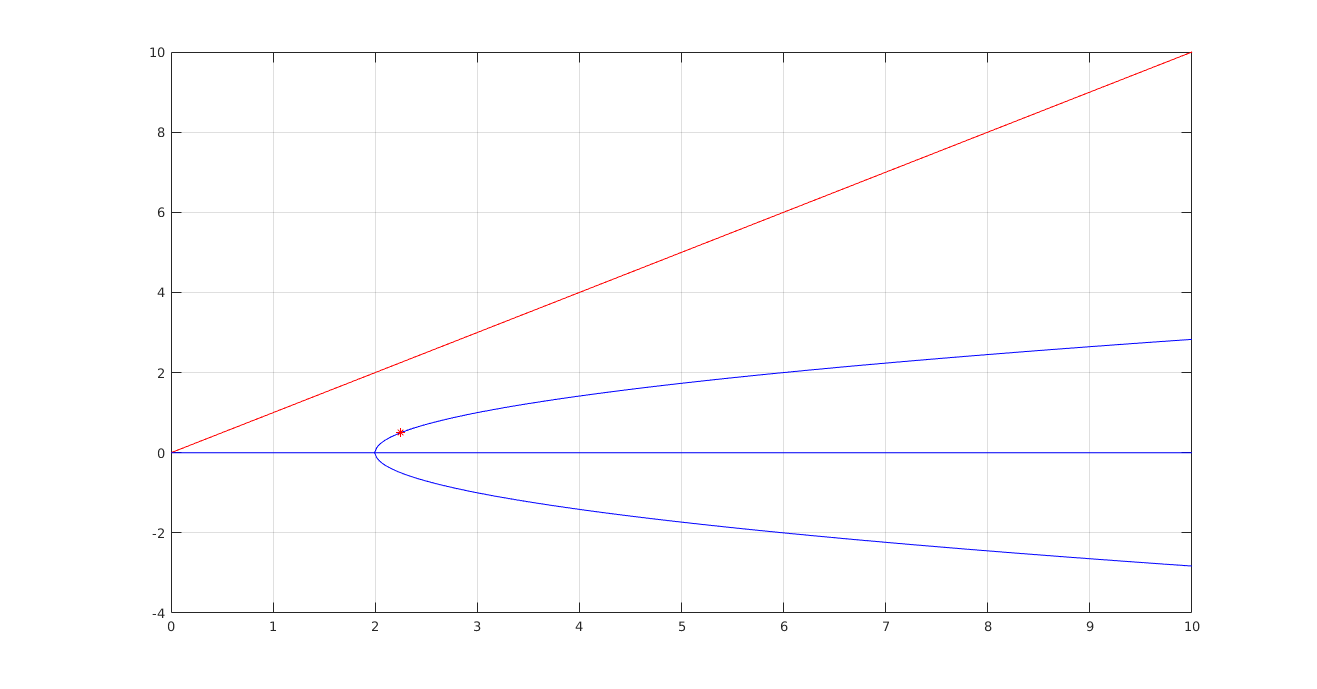
\includegraphics[scale=0.25]{plot.png}
\end{frame}

\begin{frame}{Lagrangian Multipliers}
  \begin{itemize}
  \item {
 \begin{align}
\min_x
  \frac{1}{2}x^T\begin{pmatrix}
		1 & -1\\
		-1 & 1
		\end{pmatrix}x
 \end{align}
 with constraints

  \begin{align}	
  x^{T}\begin{pmatrix}
		0 & 0\\
		0 & 1
		\end{pmatrix}x-\begin{pmatrix}
		1 & 0
		\end{pmatrix}x+2 \leq 0
 \end{align}
  }
 \end{itemize}

\end{frame}


\begin{frame}{Lagrangian Multipliers}
  \begin{itemize}
  \item {
  Lagrangian is,
 \begin{align}
 L(x,\lambda)= 
  \frac{1}{2}x^T\begin{pmatrix}
		1 & -1\\
		-1 & 1
		\end{pmatrix}x + \lambda
  \begin{pmatrix}
  x^{T}\begin{pmatrix}
		0 & 0\\
		0 & 1
		\end{pmatrix}x-\begin{pmatrix}
		1 & 0
		\end{pmatrix}x+2 
	\end{pmatrix}
 \end{align}

  }
 \end{itemize}

\end{frame}



\begin{frame}{Lagrangian Multipliers}
  \begin{itemize}
  \item {
  Lagrangian is,
 \begin{align}
 \frac{\partial L(x,\lambda)}{\partial x} = 
  \begin{pmatrix}
		1 & -1\\
		-1 & 1
		\end{pmatrix}x + \lambda
  \begin{pmatrix}
  2\begin{pmatrix}
		0 & 0\\
		0 & 1
		\end{pmatrix}x-\begin{pmatrix}
		1 & 0
		\end{pmatrix} 
	\end{pmatrix} = 0
 \end{align}
 solving,
 
 \begin{align}
 x = \begin{pmatrix}
		\lambda + 0.5\\ 0.5
		\end{pmatrix} 
 \end{align}

  }
 \end{itemize}

\end{frame}

\begin{frame}{Lagrangian Multipliers}
  \begin{itemize}
  \item {
  Lagrangian is,
 \begin{align}
 \frac{\partial L(x,\lambda)}{\partial \lambda} = x^{T}\begin{pmatrix}
		0 & 0\\
		0 & 1
		\end{pmatrix}x-\begin{pmatrix}
		1 & 0
		\end{pmatrix}x+2=0
 \end{align}
 Sub (16) in (17), and solving,
 \begin{align}
 \frac{7}{4} - \lambda = 0\\
 \lambda = \frac{7}{4}\\
  x = \begin{pmatrix}
		\frac{7}{4} + 0.5\\ 0.5
		\end{pmatrix} 
 \end{align}
X = [2.25,0.5]\\ 
Shortest distance =  1.2374\\
  }
 \end{itemize}

\end{frame}
\end{document}


